\documentclass[journal]{IEEEtran}
\usepackage{cmap}
\usepackage{amsmath}
\usepackage{amsfonts}
\usepackage{subfigure}
\usepackage[final]{graphicx}
\usepackage{graphics,picture}
\usepackage{algorithm}
\usepackage{algorithmic}
\usepackage{mathrsfs}
\usepackage{cases}
\usepackage{bm, comment,color,amssymb}
\usepackage{cite,epstopdf}
\renewcommand{\thefootnote}{\arabic{footnote}}
\newcommand{\trace}{\mathop{\mathrm{Tr}}}%\trace
\newcommand{\vectorize}{\mathop{\mathrm{vec}}}%\vectorization

\begin{document}
	
\title{Joint Spectrum Leasing and Power Allocation Optimization of Virtual Mobile Network}
	
\author{Miao Jiang, Yiqing Li, Qi Zhang, \emph{Member}, \emph{IEEE}, and Jiayin Qin

\thanks{This work was supported in part by the National Natural Science Foundation of China under Grant 61672549 and Grant 61472458, and in part by the Guangzhou Science and Technology Program under Grant 201607010098 and Grant 201804010445.

M. Jiang, Y. Li, and Q. Zhang are with the School of Electronics and Information Technology, Sun Yat-sen University, Guangzhou 510006, Guangdong, China (e-mail: jmiao@mail2.sysu.edu.cn, liyiq5@mail2.sysu.edu.cn, zhqi26@mail.sysu.edu.cn). J. Qin is with the School of Electronics and
Information Technology, Sun Yat-sen University, Guangzhou 510006, Guangdong,  China, and also with the Xinhua College, Sun Yat-sen University, Guangzhou 510520, Guangdong, China (e-mail: issqjy@mail.sysu.edu.cn). }
}% <-this % stops a space
	
	
\markboth{Submitted to IEEE Transactions on Vehicular Technology}
{Jiang \MakeLowercase{\textit{et al.}}: Joint Spectrum Leasing and Power Allocation Optimization of Virtual Mobile Network}
	
\maketitle
\begin{abstract}
Unmanned aerial vehicle (UAV) enabled communications are promising solution to provide reliable and cost-effective wireless communications
for ground users. In this paper, we consider a UAV enabled wireless powered communication network where a UAV with constant power supply first charges all users by transmitting wireless energy to all users in the downlink simultaneously and then all users send their independent information to the UAV in the uplink by time-division multiple access. Our goal is to maximize the uplink sum achievable rate of all users by jointly optimizing the time allocation as well as the position of the UAV. To solve this non-convex problem, we first derive the closed-form optimal solution of the time allocation which is expressed as the function of UAV position. The original problem, after substituting the derived optimal time allocation, is reformulated as a new optimization problem whose optimization variable is only UAV position. We propose a sequential unconstrained convex minimization based algorithm to obtain the globally optimal solution. Simulation results demonstrate that the performance of our proposed algorithm matches with that obtained by two-dimensional exhaustive search. To reduce the computational complexity, we also propose a Dinkelbach based algorithm to obtain the locally optimal solution. Simulation results show that the performances of our proposed two algorithms are superior to the schemes without time allocation optimization and/or position optimization.
\end{abstract}
\begin{IEEEkeywords} Unmanned aerial vehicle (UAV), wireless powered communication network, sequential unconstrained convex minimization, Dinkelbach.
\end{IEEEkeywords}
\IEEEpeerreviewmaketitle
	
\section{introduction}

QoS  survey the alternating direction method of multipliers (ADMM)
\section{System Model and Problem Formulation}

Consider a wireless communication system with one MNO (mobile network operator) and $N$ VMNOs (virtual mobile network operators). With wireless network virtualization operation, the whole communication processes are divided into two stages. VMNOs will first rent wireless spectrum from the MNO and then provide customized services to their MUs (mobile users) in respective service cell. Particularly, we investigate a OFDMA (orthogonal frequency division multiple access) downlink transmission scenario, where the total bandwidth owned by MNO is $W_{sum}$ Hertz (Hz). 

During the first transmission stage, the bandwidth occupied by the $i$-th VMNO is denoted as $w_i$. Thus, we have

\begin{align}
\sum_{i = 0}^{N} w_i \leq W_{sum}.
\end{align}
In this paper, without loss of generality, we assume that the $i$-th VMNO is located as the origin $o_i$. The locations of MUs are modeled as a realization of a Poisson point process (PPP) with intensity $\lambda_i$ in a fixed circular region $\mathcal{D}(o_i, r_i) \in \mathbb{R}^2$, where $r_i$ denotes the cell radius. The locations of MUs associated with the $i$-th VMNO are denoted as $\mathcal{X} = \{\mathbf{x}_{ij} \in \mathbb{R}^2 | j = 1, \cdots, N_i\}$, where $N_i = \pi r_i^2 \lambda_i$ is the expected number of MUs in the $i$-th VMNO. Note that the user set $\mathcal{X}$ changes with user arrivals, departure, or movements.

Suppose that transmitted signals are affected by both large-scale path loss and fast Rayleigh fading. Thus, the channel between the $j$-th MU and its associated $i$-th VMNO is denoted by $h_{ij} = \frac{g_{ij}}{\sqrt{1 + {\left\| \mathbf{x}_{ij} \right\|}^\alpha}}$, where $\alpha$ denotes the path-loss decay factor  and $g_{ij}$ denotes the Rayleigh fading channel state information (CSI), i.e., $g_{ij}$ is a complex Gaussian random variable with zero mean and unit variance. The instantaneous data rate for the $j$-th MU in the $i$-th VMNO is given by
\begin{align}
	R_{ij} = b_{ij}\log_2\left(1 + \frac{q_{ij} \left|h_{ij} \right|^2 }{\Gamma b_{ij}n_0}\right)
\end{align}
where $b_{ij}$ denotes the bandwidth of the $j$-th MU allocated by the $i$-th VMNO, $q_{ij}$ denotes the power allocated to the $j$-th MU by the $i$-th VMNO. $\Gamma$ denotes the SNR gap to the information theoretical channel capacity owing to the
non-ideal coding and modulation in practice \cite{JGDForney}. $n_0$ denotes the power spectral density of white noise at the MU.                      
\begin{figure}
	\centering
	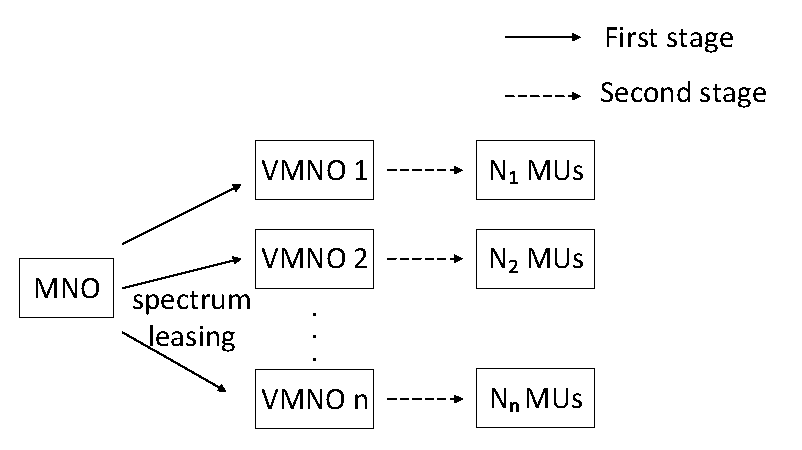
\includegraphics[width=3.6in]{Pic1.eps}
	\caption{Two-stage spectrum leasing network. During the first stage, VMNOs rent spectrum from an MNO based on the arrival rate and QoS of MUs. During the second stage, each VMNO allocates the obtained spectrum dynamically to a set of MUs.}
\end{figure}

The two-stage spectrum leasing processes are operated in two timescales, namely a period and a time slot. As shown in Fig. 1, the first stage is operated in a period and often measured in hours, where each VMNO rents wireless spectrum from a MNO. The second stage is operated in a time slot and often measured in milliseconds, during which the  wireless channel fading remains constant but may change from one time slot to anther. Notice that VMNOs will not release the occupied spectrum until the end of the whole transmission. We will discuss these two stages in the following two sections.

\section{Spectrum leasing and power allocation during the first stage}

\subsection{Problem formulation}
During the first stage, the CSI of each MU in each VMNO is a random variable. So, we first assume that the bandwidth and power allocated to all MUs in each VMNO are equal. Thus, the expected data rate of the $j$-th MU in the $i$-th VMNO is expressed as
\begin{align}
E\left({R}_{ij}\right) = \int_{0}^{\infty} \frac{w_i}{n_i} \log_2\left(1 + \frac{p_i x}{w_i n_0}\right) f_{\left|h_{ij} \right|^2} \left(x\right)dx
\end{align}
where $P_i$ denotes the total transmission power budget for the $i$-th VMNO, $f_{\left|h_{ij} \right|^2} \left(x\right)$ is the probability density function (PDF) of the random variable $\left|h_{ij} \right|^2$. 

During the first stage, we aim at minimizing the total transmit power at VMNOs under the QoS requirement at each MU in each VMNO and the total bandwidth constraint at the MNO by properly choosing the transmit power $p_i$ and the bandwidth $w_i$. Thus, the optimization problem is formulated as
\begin{subequations}\label{q4}
	\begin{align}
	\min_{\mathbf{p}, \mathbf{w}}\ & \sum\limits_{i = 1}^{N} p_i \\ \mbox{s.t.} \quad &  \sum\limits_{i = 1}^{N} w_i \leq W_{sum}\\ \quad &  E\left({R}_{ij}\right) \geq \bar{R}_i, \ p_i \geq 0, w_i \geq 0, \ \forall i, 
	\end{align}
\end{subequations}
where $\bar{R}_i$ denotes the data rate threshold at the $i$-th VMNO  \footnote{Note that in this paper, we assume that the data rate thresholds at different MUs which associated with the same VMNO are equal due to the same distribution of different MUs in each VMNO.}, $\mathbf{p} = \left[p_1, p_2, \cdots, p_N\right]^T$, $\mathbf{w} = \left[w_1, w_2, \cdots, w_N\right]^T$. To proceed, we will first introduce the following proposition:

\textit{Proposition 1}: The cumulative distribution function (CDF) of $\left|h_{ij} \right|^2$ is $F_{\left|h_{ij} \right|^2}\left(x\right) = 1 - M\left(\frac{2}{\alpha}, 1 + \frac{2}{\alpha}, - x r_i^{\alpha}\right)e^{-x}$, where $M\left(a,b,z\right)$ denotes the Kummer's function \cite{MAbramowitz}.


\textit{Proof}: See Appendix A.  $\hfill\blacksquare$

Using the above proposition 1, $f_{\left|h_{ij} \right|^2} \left(x\right)$ can be calculated as follows:
\begin{align}
&f_{\left|h_{ij} \right|^2} \left(x\right)\nonumber \\ &= \frac{d F_{\left|h\right|_{ij}^2}\left(x\right)}{d x} \nonumber \\
&=M\left(\frac{2}{\alpha}, 1 + \frac{2}{\alpha}, -xr_i^{\alpha}\right)e^{-x} -\frac{d M\left(\frac{2}{\alpha}, 1 + \frac{2}{\alpha}, -x r_i^{\alpha}\right)}{d x} e^{-x} \nonumber \\
&\overset{\left(d\right)}{=} M\left(\frac{2}{\alpha}, 1 + \frac{2}{\alpha}, -xr_i^{\alpha}\right)e^{-x} + \nonumber \\ & \quad \ \frac{2}{2+\alpha}M\left(1 + \frac{2}{\alpha}, 2+\frac{2}{\alpha}, -xr_i^{\alpha}\right)r_i^{\alpha}e^{-x} \nonumber \\
& = e^{-x}g\left(x\right)
\end{align}
where $\left(d\right)$ follows from $\frac{d M\left(a, b, z\right)}{d x} = \frac{a}{b}M\left(a+1, b+1, z\right)$ \cite[13.4.8]{MAbramowitz}, $g\left(x\right)$ is defined as follows:
\begin{align}
g\left(x\right) =& \frac{2r_i^{\alpha}}{2+\alpha} M\left(1 + \frac{2}{\alpha}, 2+ \frac{2}{\alpha}, -xr_i^{\alpha}\right) + \nonumber \\ & M\left(\frac{2}{\alpha}, 1 + \frac{2}{\alpha}, -xr_i^{\alpha}\right).
\end{align}

Now, the original optimization problem \eqref{q4} can be reformulated as follows:
\begin{subequations}\label{q7}
	\begin{align}
	\min_{\mathbf{p}, \mathbf{w}}\ & \sum\limits_{i = 1}^{N} p_i \label{q7a} \\ \mbox{s.t.} \quad &  \sum\limits_{i = 1}^{N} w_i \leq W_{sum} \label{q7b} \\ \quad &  \int_{0}^{\infty} \frac{w_i}{n_i} \log_2\left(1 + \frac{p_i x}{w_i n_0}\right) e^{-x}g\left(x\right) dx \geq \bar{R}_i, \forall i \label{q7c}\\
	& p_i \geq 0, w_i \geq 0, \ \forall i, \label{q7d}
	\end{align}
\end{subequations}
it is observed in \eqref{q7c}, the calculation of the integration is complicated and can be calculated via numerical integration. Denote the left-hand sides (LHSs) of \eqref{q7c} as $q\left(p_i, w_i\right)$. The numerical integration can be very time-consuming when the integrand of $\kappa\left(p_i, w_i\right)$ has a heavy tail. Thus, next we will apply half-range Gauss-Hermite Quadrature (HR-GHQ) to approximate $q\left(p_i, w_i\right)$ with high accuracy \cite{JSBall,NMSteen}.

Based on \cite{NMSteen}, a $K$-point HR-GHQ can be written as
\begin{align} \label{q8}
\int_{0}^{\infty}e^{-x^2} f\left(x\right) dx \approx \sum\limits_{k = 1}^{K} a_k f\left(x_k\right)
\end{align}
where both the weights $\{a_k\}_{k = 1}^K$ and abscissas $\{x_k\}_{k = 1}^K$ are real numbers. After applying \eqref{q8} to $\kappa \left(p_i, w_i\right)$, we have

\begin{align} \label{q9}
\kappa \left(p_i, w_i\right) &\overset{\left(e\right)}{=} \int_{0}^{\infty}e^{-t^2}\frac{w_i}{n_i} g\left(t^2\right) 2t \log_2\left(1 + \frac{p_it^2}{w_in_0}\right)dt  \nonumber \\
& \overset{\left(f\right)}{\approx} \sum\limits_{i = 1}^{K_i}a_{ki}\frac{w_i}{n_i}g\left(t_{ki}^2\right)2t_{ki}\log_2\left(1 + \frac{p_it_{ki}^2}{w_in_0}\right) \nonumber \\
& \overset{\left(g\right)}{=} \sum\limits_{k = 1}^{K_i}b_{ki}\frac{w_i}{n_i}\log_2\left(1 + \frac{p_it_{ki}^2}{w_in_0}\right)
\end{align}
where $\left(e\right)$ follows from $x = t^2$, $\left(f\right)$ follows from \eqref{q8}, $\left(g\right)$ follows from $b_{ki} = a_{ki}g\left(t_{ki}^2\right)2t_{ki}$.

Finally, the spectrum leasing allocation optimization problem can be expressed as follows:
\begin{subequations}\label{q10}
	\begin{align}
	\min_{\mathbf{p}, \mathbf{w}}\ & \sum\limits_{i = 1}^{N} p_i \label{q10a} \\ \mbox{s.t.} \quad &  \sum\limits_{i = 1}^{N} w_i \leq W_{sum} \label{q10b} \\ \quad &  \sum\limits_{k = 1}^{K_i}b_{ki}\frac{w_i}{n_i}\log_2\left(1 + \frac{p_it_{ki}^2}{w_in_0}\right) \geq \bar{R}_i, \forall i \label{q10c}\\
	& p_i \geq 0, w_i \geq 0, \ \forall i. \label{q10d}
	\end{align}
\end{subequations}
Since problem \eqref{q10} is convex in terms of optimization variables $\mathbf{p}$ and $\mathbf{w}$, it can be solved efficiently by existing optimization tools such as CVX \cite{SBoyd1}. Next, we will exploit the structure of problem \eqref{q10} and obtain its global optimal solution via using a distributed algorithm named ADMM \cite{SBoyd2,EChen} to further reduce the complexity.
\subsection{ADMM-based distributed algorithm for solving optimization problem \eqref{q10}}
First, we will introduce an auxiliary variable $\mathbf{z} = \left[z_1, z_2, \cdots, z_N\right]^T$. Thus, optimization problem \eqref{q10} can be reformulated as

\begin{subequations}\label{eq11}
	\begin{align}
	\min_{\mathbf{p}, \mathbf{w}, \mathbf{z}}\ & \sum\limits_{i = 1}^{N} p_i \label{eq11a} \\ \mbox{s.t.} \quad &  \mathbf{w} - \mathbf{z} = \mathbf{0} \label{eq11b} \\ \quad &  \sum\limits_{i = 1}^{N}z_i \leq W_{sum} \label{eq11c} \\ \quad &  \sum\limits_{k = 1}^{K_i}b_{ki}\frac{w_i}{n_i}\log_2\left(1 + \frac{p_it_{ki}^2}{w_in_0}\right) \geq \bar{R}_i, \forall i \label{eq11d}\\
	& p_i \geq 0, w_i \geq 0, z_i \geq 0, \ \forall i. \label{eq11e}
	\end{align}
\end{subequations}

Denote the feasible region of constraint \eqref{eq11c} and $z_i \geq 0, \forall i$ as $\mathcal{C}$, its indicator function can be defined as
\begin{equation}
\mathbb{I}_\mathcal{C}\left(\mathbf{z}\right) = \left\{ \begin{array}{lcl}
0, & &\mbox{if} \ \mathbf{z} \in \mathcal{C}, \\
+\infty, & &\mbox{otherwise}.
\end{array}
\right.
\end{equation}
Likewise, denote the feasible region of constraint \eqref{eq11d}, $p_i\geq 0$ and $w_i \geq 0, \forall i$ as $\mathcal{D}$, its indicator function can be defined as
\begin{equation}
\mathbb{I}_\mathcal{D}\left(\mathbf{p},\mathbf{w}\right) = \left\{ \begin{array}{lcl}
0, & &\mbox{if} \ \left(\mathbf{p}, \mathbf{w}\right) \in \mathcal{D}, \\
+\infty, & &\mbox{otherwise}.
\end{array}
\right.
\end{equation}
Thus, problem \eqref{eq11} can be rewritten in ADMM form as follows:
\begin{subequations}\label{eq14}
	\begin{align}
	\min_{\mathbf{p}, \mathbf{w}, \mathbf{z}}\ & \sum\limits_{i = 1}^{N} p_i + \mathbb{I}_\mathcal{C}\left(\mathbf{z}\right) + \mathbb{I}_\mathcal{D}\left(\mathbf{p},\mathbf{w}\right)  \label{eq14a} \\ \mbox{s.t.} \quad &  \mathbf{w} - \mathbf{z} = \mathbf{0} \label{eq14b}
	\end{align}
\end{subequations}
Then, the augmented Lagrangian (using the scaled dual variable) of problem \eqref{eq14} is given by
\begin{align}
\mathcal{L}_\rho\left(\mathbf{p},\mathbf{w}, \mathbf{z},\mathbf{u}\right) = & \sum\limits_{i = 1}^{N} p_i + \mathbb{I}_\mathcal{C}\left(\mathbf{z}\right) + \mathbb{I}_\mathcal{D}\left(\mathbf{p},\mathbf{w}\right) + \\ & \frac{\rho}{2}\left\|\mathbf{w} - \mathbf{z} + \mathbf{u}\right\|_2^2
\end{align}
where $\rho > 0$ is the penalty parameter and $\mathbf{u} = [u_1, u_2, \cdots, u_N]^T$ is the dual variable for the  constraint \eqref{eq14b}. From problem \eqref{eq14}, it can be observed that the variables can be split into two blocks: $\{\mathbf{p}, \mathbf{w}\}$ and $\mathbf{z}$. Besides, the objective function is also separable across this splitting. Therefore, the ADMM technique can be applied to solve this problem by iteratively updating $\{\mathbf{p}, \mathbf{w}\}$, $\mathbf{z}$ and $\mathbf{u}$. Denote the values in the $k$-th iteration as $\{\mathbf{p}^k, \mathbf{w}^k, \mathbf{z}^k, \mathbf{u}^k\}$. Thus, in the $(k+1)$-th iteration, the variables can be updated sequentially as follows:
 
1) step 1: Given $\{\mathbf{z}^k, \mathbf{u}^k\}$, we first maximize $\mathcal{L}_\rho$ with respect to $\{\mathbf{p}, \mathbf{w}\}$, where
\begin{align}
\{\mathbf{p}^{k+1}, \mathbf{w}^{k+1}\} = \arg \max_{\mathbf{p}, \mathbf{w}} \mathcal{L}_\rho\left(\mathbf{p}, \mathbf{w}, \mathbf{z}^k, \mathbf{u}^k\right) \label{q17}
\end{align}
Notice that the update of $\mathbf{p}$ and $\mathbf{w}$ in problem \eqref{q17} is equivalent to solving the following problem:
\begin{subequations}\label{eq18}
	\begin{align}
	\min_{\mathbf{p}, \mathbf{w}}\ & \sum\limits_{i = 1}^{N} p_i + \frac{\rho}{2}\sum\limits_{i = 1}^{N}\left(w_i - z_i^k + u_i^k \right)^2  \label{eq18a} \\ \mbox{s.t.} \quad &  \eqref{eq11d},  \label{eq18b} \\
	& w_i\geq 0, p_i \geq 0, \forall i. \label{eq18c}
	\end{align}
\end{subequations}
It is observed that problem \eqref{eq18} can be decomposed into $N$ subproblems, each subproblem solves:
\begin{subequations}\label{eq19}
	\begin{align}
	\min_{p_i, w_i}\ & p_i + \frac{\rho}{2}\left(w_i - z_i^k + u_i^k \right)^2  \label{eq19a} \\ \mbox{s.t.} \quad & \sum\limits_{k = 1}^{K_i}b_{ki}\frac{w_i}{n_i}\log_2\left(1 + \frac{p_it_{ki}^2}{w_in_0}\right) \geq \bar{R}_i,  \label{eq19b} \\
	& w_i\geq 0, p_i \geq 0. \label{eq19c}
	\end{align}
\end{subequations}
Notice that each subproblem \eqref{eq19} is a convex problem and can be solved efficiently using interior point method \cite{SBoyd3}.

2) step 2: Given $\{\mathbf{p}^{k+1}, \mathbf{w}^{k+1}, \mathbf{u}^k\}$, we then maximize $\mathcal{L}_\rho$ with respect to $\mathbf{z}$, where
\begin{align}
\mathbf{z} = \arg \max_{\mathbf{z}} \mathcal{L}_\rho\left(\mathbf{p}^{k+1}, \mathbf{w}^{k+1}, \mathbf{z}, \mathbf{u}^k\right),
\end{align} 
which can be equivalently written as the following convex optimization problem: 
\begin{subequations}\label{eq21}
	\begin{align}
	\min_{\mathbf{z}}\ & \left\|\mathbf{w}^{k+1} - \mathbf{z} + \mathbf{u}^k \right\|_2^2 \label{eq21a} \\ \mbox{s.t.} \quad & \left\|\mathbf{z} \right\|_1 \leq W_{sum},  \label{eq21b} \\
	& z_i\geq 0, \forall i. \label{eq21c}
	\end{align}
\end{subequations}
The above convex problem \eqref{eq21} is the $l_1$ ball problem \cite{JDuchi} and we can obtain its closed-form solution as follows:

(a) If $\left\|\mathbf{w}^{k+1} + \mathbf{u}^k \right\|_1 > W_{sum}$, $z_i^{k+1}$ can be obtained as follows:
\begin{align} \label{eq22}
z_i^{k+1} = \max\left\{w_i^{k+1} + u_i^k - \beta, 0\right\}
\end{align}
where $\beta = \frac{1}{\zeta}\left(\sum\limits_{i = 1}^{\zeta} v_i - W_{sum} \right)$, $\mathbf{v} = \left[v_1, v_2, \cdots, v_N\right]^T$ and $\mathbf{v}$ denotes the vector obtained by sorting $\mathbf{w}^{k+1} + \mathbf{u}^k$ in a descending order. $\zeta$ is denoted as 
\begin{align}
\zeta = \max_{1 \leq i \leq N} \left\{ i \left| v_i - \frac{1}{i}\left(\sum\limits_{j = 1}^{i} v_j - W_{sum}\right) > 0 \right. \right\}
\end{align}

(b) If $\left\|\mathbf{w}^{k+1} + \mathbf{u}^k \right\|_1 \leq W_{sum}$, $z_i^{k+1}$ can be obtained as
\begin{align}
z_i^{k+1} = w_i^{k+1} + u_i^k
\end{align}

3) step 3: Given $\{\mathbf{w}^{k+1}, \mathbf{z}^{k+1}\}$, we minimize $\mathcal{L}_\rho$ with respect to $\mathbf{u}$, which is achieved
by updating the dual variable $\mathbf{u}$ as
\begin{align} \label{eq25}
\mathbf{u}^{k+1} =\mathbf{w}^{k+1} - \mathbf{z}^{k+1} + \mathbf{u}^k
\end{align}
\begin{algorithm}[h]
	\caption{The proposed ADMM based method for solving problem \eqref{q10}.}
	\begin{algorithmic}[1]
		\STATE \textbf{Initialize:} $w_i^0 = \frac{W_{sum}}{N_i}$, $p_i^0$, $z_i^0 = 0$, and $u_i^0 = 0$, $\forall i$. $k = 0$. Set the penalty parameter $\rho = 1$. \STATE
		\textbf{Repeat:} \\
		Each VMNO updates its local variables $\{w_i^{k+1}, p_i^{k+1}\}$ by solving \eqref{eq19} in parallel and the obtained results $\{w_i^{k+1}\}$ are passed to the MNO;\\
		The MNO updates the variable $\mathbf{z}^{k+1}$ with closed-form expression \eqref{eq22};\\
		The MNO updates the dual variable $\mathbf{u}^{k+1}$ using \eqref{eq25};\\
		$k:=k+1$;\\
		\STATE \textbf{Until:} convergence.
	\end{algorithmic}
\end{algorithm}

\section{Dynamic spectrum allocation and power allocation during the second stage}
During the second stage, each VMNO dynamically allocates the spectrum that has already been rent from MNO during the first stage to MUs in its serving region. The resource allocation can be performed during different time slots at the second stage and we only focus on a particular time slot. We further assume that perfect CSIs can be estimated by each VMNO at each time slot. Thus, the resource allocation optimization problem in the $i$-th VMNO can be formulated as
\begin{subequations}\label{q11}
	\begin{align}
	\min_{q_{ij}, b_{ij}}\ & \sum\limits_{j = 1}^{N_i} q_{ij} \label{q11a} \\ \mbox{s.t.} \quad &  \sum\limits_{j = 1}^{N_i} b_{ij} \leq w_i \label{q11b} \\ \quad &  b_{ij}\log_2\left(1 + \frac{q_{ij}\left|h_{ij}\right|^2}{b_{ij}n_0}\right) \geq \tilde{R}_i, \forall j \label{q11c}\\
	& q_{ij} \geq 0, b_{ij} \geq 0, \ \forall j, \label{q11d}
	\end{align}
\end{subequations}
where $\tilde{R}_i$ denotes the QoS requirement of MUs in the $i$-th VMNO.

\textit{Lemma 1}: For problem \eqref{q11}, the optimal variables $q_{ij}$ and $b_{ij}$ should satisfy that the QoS constraints in \eqref{q11c} are all active, i.e., 
\begin{align}
b_{ij}\log_2\left(1 + \frac{q_{ij}\left|h_{ij}\right|^2}{b_{ij}n_0}\right) = \tilde{R}_i,  \forall j
\end{align}

\textit{Proof}:  
We prove Lemma 1 by reductio ad absurdum. Assume that $q_{ij}^o, \forall j$ are the optimal solutions to \eqref{q11} such that $b_{ij}\log_2\left(1 + \frac{q_{ij}^o\left|h_{ij}\right|^2}{b_{ij}n_0}\right) > \tilde{R}_i, \forall j$. Define a set of $\Delta q_{ij} > 0, \forall j$ such that 
\begin{align}
b_{ij}\log_2\left(1 + \frac{q_{ij}^o\left|h_{ij}\right|^2}{b_{ij}n_0}\right) > b_{ij}\log_2\left(1 + \frac{q_{ij}^\dag\left|h_{ij}\right|^2}{b_{ij}n_0}\right), \forall j
\end{align}
where $q_{ij}^\dag = q_{ij}^o - \Delta q_{ij}, \forall j$. Therefore, we can choose $\Delta q_{ij}$ appropriately such that $b_{ij}\log_2\left(1 + \frac{q_{ij}^\dag\left|h_{ij}\right|^2}{b_{ij}n_0}\right) = \tilde{R}_i, \forall j$. It is note that $q_{ij}^\dag, \forall j$ are feasible and have smaller objective function value than $q_{ij}^o, \forall j$.
$\hfill\blacksquare$

Combined with Lemma 1, problem \eqref{q11} can be equivalently written as follows:
\begin{subequations}\label{q14}
	\begin{align}
	\min_{b_{ij}}\ & \sum\limits_{i = 1}^{N_i} \frac{b_{ij}n_0}{\left|h_{ij}\right|^2}\left(2^{\frac{\tilde{R}_i}{b_{ij}}} - 1\right) \label{q14a} \\ \mbox{s.t.} \quad &  \sum\limits_{j = 1}^{N_i} b_{ij} \leq w_i \label{q14b} \\
	& b_{ij} \geq 0, \ \forall j. \label{q14c}
	\end{align}
\end{subequations}
Problem \eqref{q14} is convex and can be solved by convex optimization techniques. We can obtain the optimal spectrum allocation solution for \eqref{q14} using the following proposition:

\textit{Proposition 2} : The optimal spectrum allocation solution for \eqref{q14}, denoted by $b_{ij}^\star$, is
\begin{align}
b_{ij}^\star = \frac{\hat{R}_i}{1 + \mathcal{W}_0\left(\frac{\mu^{\star}\left|h_{ij}\right|^2 - n_0}{en_0}\right)}, \forall j,
\end{align}
where $\hat{R}_i = \tilde{R}_i\ln2$, $\mathcal{W}_0\left(\phi\right)$ is the branch satisfying $\mathcal{W}\left(\phi\right) \geq -1$ and $\mathcal{W}$ denotes the Lambert $\mathcal{W}$ function of $\phi$ \cite{RMCorless}, $\mu^{\star} > 0$ is a constant and can be obtained by using one-dimension (1-D) bisection search over interval $\left[\mu_{min}, \mu_{max}\right]$ with
\begin{align}
\mu_{min} &= \frac{n_0e\left(\frac{N_i\hat{R}_i}{w_i} - 1\right)e^{\left(\frac{N_i\hat{R}_i}{w_i} - 1\right)} + n_0}{h_{max}}  \\
\mu_{max} & = \frac{n_0e\left(\frac{N_i\hat{R}_i}{w_i} - 1\right)e^{\left(\frac{N_i\hat{R}_i}{w_i} - 1\right)} + n_0}{h_{min}}
\end{align}
where $h_{max}$ and $h_{min}$ denote the maximum and minimum channel gains among $N_i$ users in the $i$-th VMNO, respectively.

\textit{Proof}: See Appendix B.  $\hfill\blacksquare$
\section{Simulation Results}
In this section, we evaluate the performance of our proposed spectrum leasing and allocation policies through numerical results. 

We consider a multicell system consisting of six circular areas ($N = 6$) and each VMNO is located at the center of the cell. The radii and the corresponding user densities of the six cells are configured as $(r_1 = 80\mbox{m}, \lambda_1 = 2400/\mbox{km}^2)$, $(r_2 = 80\mbox{m}, \lambda_2 = 1600/\mbox{km}^2)$, $(r_3 = 100\mbox{m}, \lambda_3 = 1600/\mbox{km}^2)$, $(r_4 = 100\mbox{m}, \lambda_4 = 2000/\mbox{km}^2)$, $(r_5 = 120\mbox{m}, \lambda_5 = 2000/\mbox{km}^2)$, and $(r_6 = 120\mbox{m}, \lambda_6 = 2400/\mbox{km}^2)$. Each VMNO and corresponding MUs are equipped with one antenna. MUs are randomly and uniformly distributed within each cell. All the channels from MUs to corresponding VMNO are assumed to be subjected to three components: path-loss, log-normal shadowing, and small-scale Rayleigh fading. The path-loss decay factor is 3.76, 
path-loss at reference distance 1m is 15.3dB, the standard deviation for Shadowing is 8dB and Rayleigh small scale fading is 0dB. For \eqref{q9}, we set $K_i = 500, \forall i$. In all simulations, the total transmit power of each VMNO is computed by using 10000 randomly generated channel realizations. Noise spectral density of -174dBm/Hz and 10dBi antenna gain are considered. If not specified, the total bandwidth $W_{sum}$ is set to be 100MHz and the minimum rate requirements $R_{min}$ are set as $\bar{R}_i = \tilde{R}_i = R_{min} = 1\mbox{Mbps}, \forall i$.

\begin{figure}
	\centering
	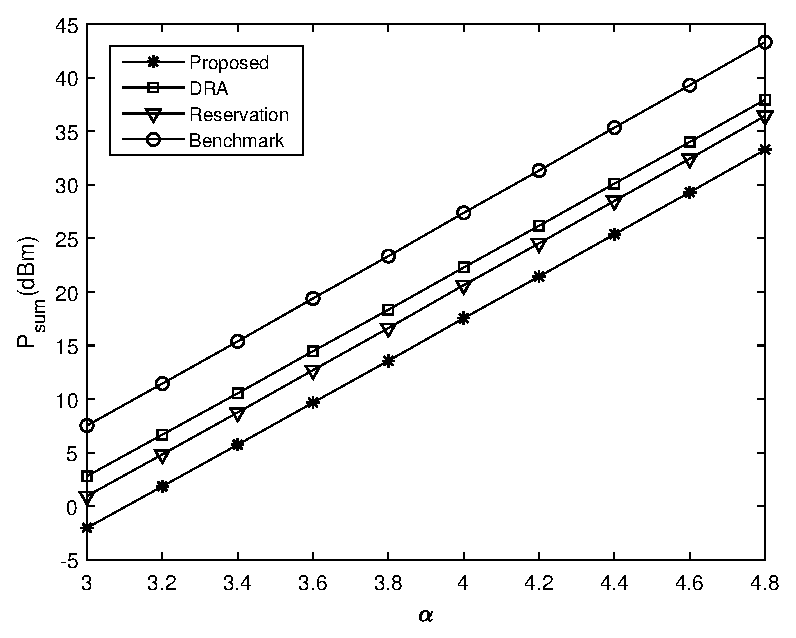
\includegraphics[width=3.6in]{P_alpha.eps}
	\caption{Total transmit power $P_{sum}$ at the six VMNOs versus the path-loss decay factor $\alpha$; performance comparison of different schemes when the total bandwidth is 100MHz and the minimum rate requirement $R_{min}$ is 1Mbps.}
\end{figure}
In Fig. 2, we present the total transmit power $P_{sum}$ comparison of different schemes for different path-loss decay factors $\alpha$ when the total bandwidth is 100MHz and the minimum rate requirement $R_{min}$ is 1Mbps. Note that $P_{sum}$ is defined as the total transmit power at the six VMNOs during the second stage. In the legend, ``Proposed" denotes our proposed scheme where spectrum and power allocation factors are optimized during two stages. ``DRA" denotes the dynamic resource allocation where the spectrum and power allocation factors are only optimized during the second stage and the spectrum is equally allocated during the first stage. ``Reservation" denotes that the spectrum and power allocation factors are only optimized during the first stage and the spectrum is equally allocated during the second stage. ``Benchmark" denotes the scheme that the spectrum is equally allocated both during the first stage and the second stage. It is observed that when the path-loss decay factor $\alpha$ increases, the total transmit power $P_{sum}$ substantially increases for all the schemes. Moreover, our proposed scheme is observed to achieve notably smaller total transmit power than the others schemes, which demonstrates the effectiveness of our proposed spectrum leasing and power allocation scheme.


\begin{figure}
	\centering
	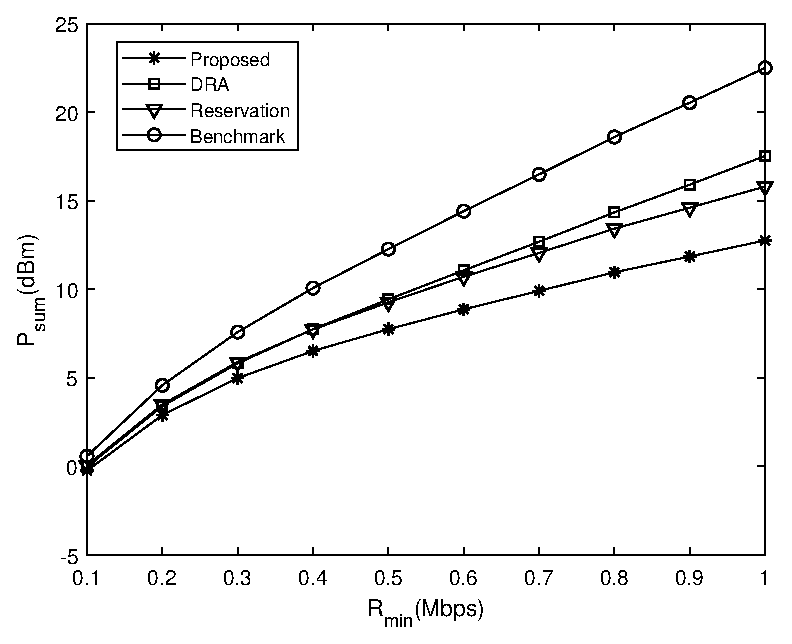
\includegraphics[width=3.6in]{P_rmin.eps}
	\caption{Total transmit power $P_{sum}$ at the six VMNOs versus the minimum rate requirement at MUs; performance comparison of different schemes when the total bandwidth is 100MHz and the path-loss decay factor is 3.76.}
\end{figure}

In Fig. 3, we present the total transmit power $P_{sum}$ comparison of different schemes for different minimum rate requirements $R_{min}$ when the total bandwidth is 100MHz and the path-loss decay factor is 3.76. Here, we assume that $\bar{R}_i = \tilde{R}_i= R_{min}, \forall i$. From Fig. 3, it is observed that as the minimum rate requirement constraint $R_{min}$ becomes more stringent, substantially more total transmit power $P_{sum}$ is needed at the six VMNOs. In particular, the performance gap between our proposed scheme and the other schemes becomes larger when the minimum rate requirements $R_{min}$ increases.

\begin{figure}
	\centering
	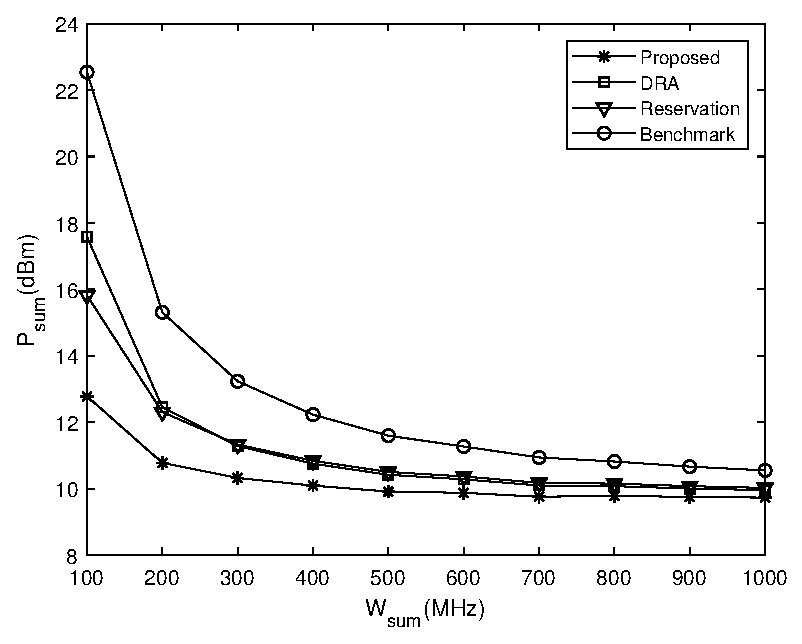
\includegraphics[width=3.6in]{P_wsum.eps}
	\caption{Total transmit power $P_{sum}$ at the six VMNOs versus the total bandwidth $W_{sum}$ owned by the MNO; performance comparison of different schemes when the minimum rate requirement is 1Mbps and the path-loss decay factor is 3.76.}
\end{figure}

In Fig. 4, we present the total transmit power $P_{sum}$ comparison of different schemes for different total bandwidth $W_{sum}$ when the minimum rate requirement is 1Mbps and the path-loss decay factor is 3.76. From Fig. 4, it is observed that as the total bandwidth $W_{sum}$ increases, the total transmit power $P_{sum}$ substantially decreases for all schemes. It is also found that our proposed scheme outperforms the other schemes.

\begin{figure}
	\centering
	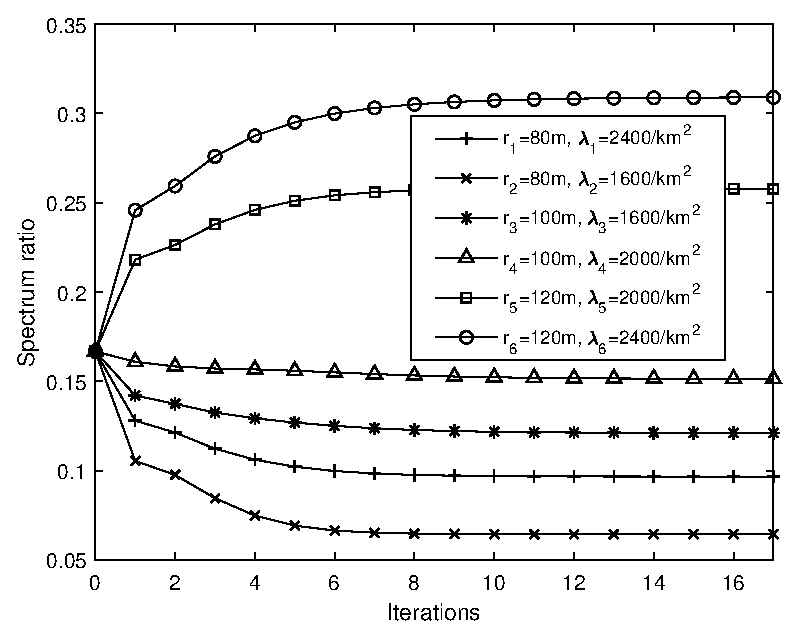
\includegraphics[width=3.6in]{SR_convergence.eps}
	\caption{Spectrum ratio versus the number of iterations at six VMNOs when the total bandwidth is 100MHz, the minimum rate requirement is 1Mbps, and the path-loss decay factor is 3.76.}
\end{figure}

In Fig. 5, we present the spectrum ratio occupied by each VMNO for different iteration times when the total bandwidth is 100MHz and the minimum rate requirement is 1Mbps, where spectrum ratio is defined as the ratio of the bandwidth occupied by the VMNO to the total bandwidth.  It is found from Fig. 2 that after only 6$\sim$8 iterations, the steady spectrum ratio is achieved. It is also found that both radius and user density in the VMNO have significant effects on the spectrum ratio. The larger the radius of the cell is configured, the more bandwidth is needed. Likewise, the larger the user density of the cell is configured, the more bandwidth is needed. 


\begin{figure}
	\centering
	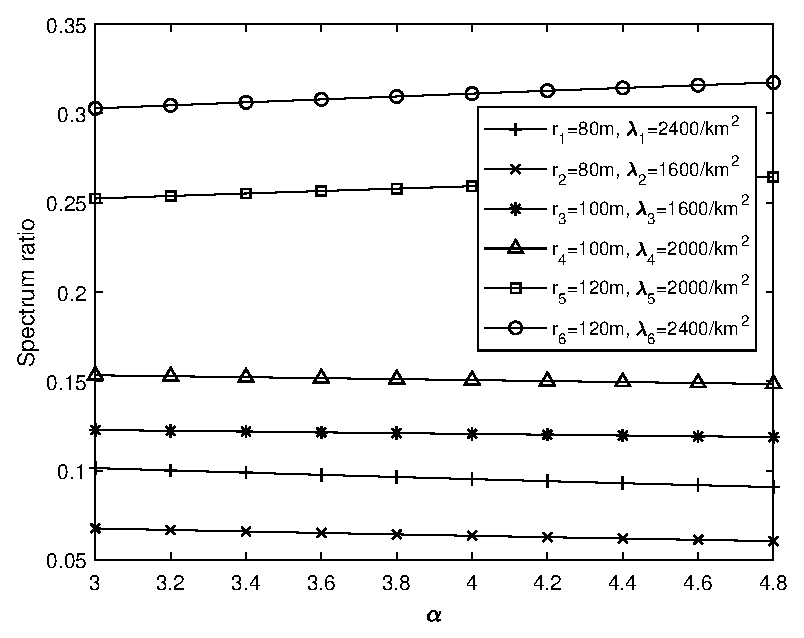
\includegraphics[width=3.6in]{SR_alpha.eps}
	\caption{Spectrum ratio versus the path-loss decay factor $\alpha$ when the minimum rate requirement is 1Mbps and the total bandwidth is 100MHz.}
\end{figure}


\begin{figure}
	\centering
	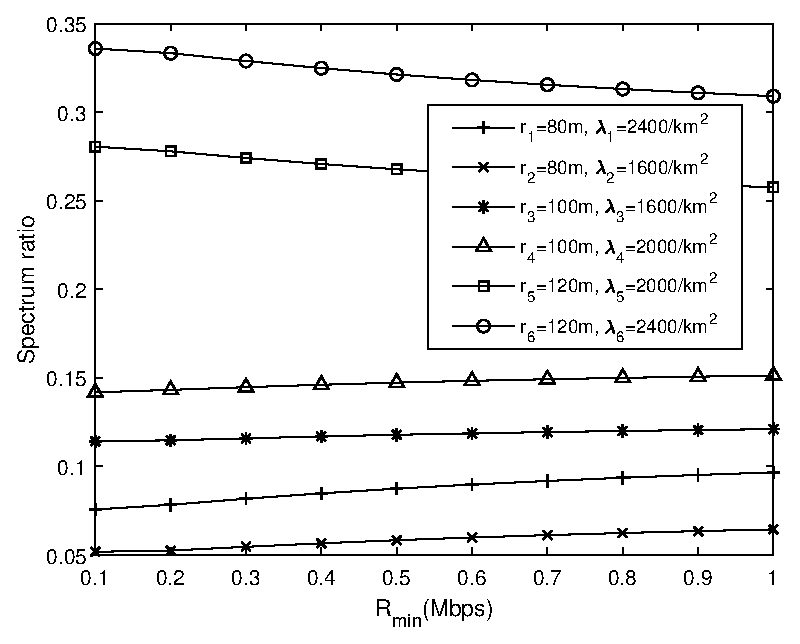
\includegraphics[width=3.6in]{SR_rmin.eps}
	\caption{Spectrum ratio versus the minimum rate requirements at six VMNOs when the total bandwidth is 100MHz and the path-loss decay factor is 3.76.}
\end{figure}


\begin{figure}
	\centering
	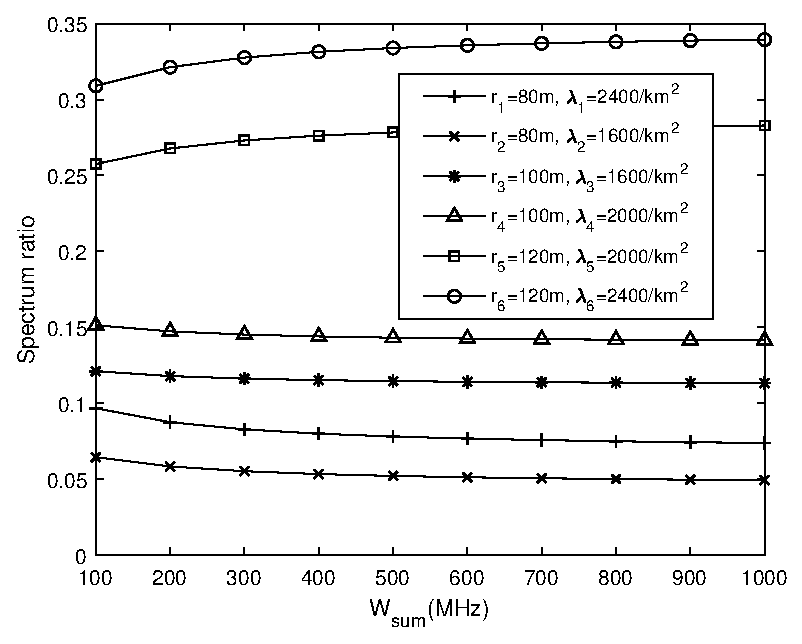
\includegraphics[width=3.6in]{SR_wsum.eps}
	\caption{Spectrum ratio versus  the total bandwidth $W_{sum}$ owned by the MNO when the minimum rate requirement is 1Mbps and the path-loss decay factor is 3.76.}
\end{figure}

\section{Conclusion}

\appendices
\section{Proof of Proposition 1}
The CDF of $\left|h_{ij} \right|^2$ is calculated as follows:

\begin{align}
F_{\left|h_{ij} \right|^2} \left(x\right) &= Prob\left(\frac{\left|g_{ij}\right|^2}{1 + d_{ij}^{\alpha}} \leq x \right) \nonumber \\
& = Prob \left(\left|g_{ij}\right|^2 \leq x \left(1 + d_{ij}^\alpha\right)\right) \nonumber \\
& \overset{\left(a\right)}{=} \int_{\mathcal{D}(o_i, r_i)} \frac{1}{\pi r_i^2}\left(1 - e^{-x\left(1 + d_{ij}^{\alpha}\right)}\right) d\Delta S \nonumber\\
& \overset{\left(b\right)}{=} \frac{1}{\pi r_i^2} \int_{0}^{r_i} \int_{-\pi}^{\pi}\left(1 - e^{-x\left(1 + y^{\alpha}\right)}\right)y d \theta d y \nonumber \\
& = \frac{2}{r_i^2}\int_{0}^{r_i} \left(y - ye^{-x\left(1 + y^\alpha\right)}\right) dy \nonumber \\
& = \frac{2}{r_i^2}\int_{0}^{r_i}y dy - \frac{2}{r_i^2}\int_{0}^{r_i} y e^{-x \left(1 + y^\alpha\right)}dy \nonumber \\
& = 1 - \frac{2}{r_i^2}e^{-x} \int_{0}^{r_i}y e^{-xy^{\alpha}}dy
\end{align}
where $\left(a\right)$ follows from the CDF of the exponential random variable $\left|g_{ij}\right|^2$, $\left(b\right)$ follows by using polar coordinates. Let $t = xy^{\alpha}$, $F_{\left|h_{ij} \right|^2} \left(x\right)$ can be further derived as follows:
\begin{align}
F_{\left|h_{ij} \right|^2} \left(x\right) &= 1 - \frac{2}{r_i^2}e^{-x} \int_{0}^{x r_i^{\alpha}} t^{\frac{1}{\alpha}} x^{-\frac{1}{\alpha}}e^{-t} d\left(t^{\frac{1}{\alpha}} x^{-\frac{1}{\alpha}}\right) \nonumber \\
& = 1 - \frac{1}{\alpha} \frac{2}{r_i^2} x^{-\frac{2}{\alpha}} e^{-x} \int_{0}^{x r_i^{\alpha}} t^{\frac{2}{\alpha} - 1}e^{-t} dt \nonumber \\
& = 1 - \frac{2}{\alpha} \left(x r_i^{\alpha}\right) ^{-\frac{2}{\alpha}} \gamma\left(\frac{2}{\alpha}, xr_i^{\alpha}\right)e^{-x} \nonumber \\
& \overset{\left(c\right)}{=} 1 - M\left(\frac{2}{\alpha}, 1 + \frac{2}{\alpha}, -xr_i^{\alpha}\right)e^{-x}
\end{align}
where $\gamma\left(s,x\right) = \int_{0}^{x}t^{s-1}e^{-t}dt$ denotes the lower incomplete gamma function, $M\left(a,b,z\right)$ denotes the Kummer's function \cite{MAbramowitz}, $\left(c\right)$ follows from $\gamma\left(s,x\right) = s^{-1} x^s M\left(s,s+1,-x\right)$. Thus the proof is completed. 

\section{Proof of Proposition 2}
The Lagrangian of problem \eqref{q14} is given by
\begin{align}
\mathcal{L}\left(b_{ij}, \mu\right) &=  \sum\limits_{i = 1}^{N_i} \frac{b_{ij}n_0}{\left|h_{ij}\right|^2}\left(2^{\frac{\tilde{R}_i}{b_{ij}}} - 1\right) + \mu\left(\sum_{j = 1}^{N_i}b_{ij} - w_i\right) \nonumber \\ 
& \overset{\left(h\right)}{=} \sum\limits_{i = 1}^{N_i} \frac{b_{ij}N_0}{\left|h_{ij}\right|^2}\left(e^{\frac{\hat{R}_i}{b_{ij}}} - 1\right) + \mu\left(\sum_{j = 1}^{N_i}b_{ij} - w_i\right) 
\end{align}
where $\mu \geq 0$ denotes the Lagrange multiplier associated with the constraint \eqref{q14b}. $\left(h\right)$ follows from $\hat{R}_i = \tilde{R}_i \ln2$. Thus, the dual function of problem \eqref{q14} is given by
\begin{align}
\mathcal{G}\left(\mu\right) = \min_{b_{ij}\geq 0} \mathcal{L}\left(b_{ij},\mu\right)
\end{align}

It can be seen from problem \eqref{q14} that there exist a set of $b_{ij}$ with $b_{ij} \geq 0$, satisfying $\sum\limits_{j = 1}^{N_i} b_{ij} \leq w_i, \forall j$. Thus, thanks to the Slater's condition, strong duality for problem \eqref{q14} holds. The Karush-Kuhn-Tucker (KKT) conditions which are both necessary and 	sufficient for the  global optimality of problem \eqref{q14} are given by
\begin{align}
\frac{\partial \mathcal{L}\left({b_{ij}^\star}, \mu^\star\right)}{\partial b_{ij}} &= 0 \label{q20} \\
\mu^\star\left(\sum\limits_{j = 1}^{N_i}b_{ij}^\star - w_i\right) &= 0 \label{q21} \\
\sum\limits_{j = 1}^{N_i}b_{ij}^\star - w_i & \leq 0 \label{q22}
\end{align} 
where $b_{ij}^\star$ and $\mu^\star$ denote the optimal primal and dual solutions of problem \eqref{q14}, respectively. It can be easily verified that $\sum\limits_{j = 1}^{N_i} b_{ij}^\star = w_i$ must hold for problem \eqref{q14}. Thus, from \eqref{q21}, we have $\mu^\star > 0$. From \eqref{q20}, it follows that 
\begin{align}
\frac{\partial \mathcal{L} \left(b_{ij}^\star, \mu^\star \right)}{\partial b_{ij}} &= \frac{n_0}{\left|h_{ij}\right|^2} \left(e^{\frac{\hat{R}}{b_{ij}^\star}} -  \frac{\hat{R}_i}{b_{ij}^\star} e^{\frac{\hat{R}_i}{b_{ij}^\star}} - 1\right) + \mu^\star \label{q24} \\
& =  \frac{n_0}{\left|h_{ij}\right|^2}\left(\left(1 - \frac{\hat{R}_i}{b_{ij}^\star}\right)e^{\frac{\hat{R}_i}{b_{ij}^\star} - 1}e - 1\right) + \mu^\star \\
& = 0. \label{q25}
\end{align}
From \eqref{q24} and \eqref{q25}, we have
\begin{align}
\left(\frac{\hat{R}_i}{b_{ij}^\star} - 1\right) e^{\frac{\hat{R}}{b_{ij}^\star} - 1} = \frac{\mu^\star \left|h_{ij}\right|^2 - n_0}{n_0 e},
\end{align}
according to the definition of Lambert $\mathcal{W}$ function, we can obtain the optimal $W_{ij}^\star$ as follows:
\begin{align}
b_{ij}^\star = \frac{\hat{R}_i}{1 + \mathcal{W}_0\left(\frac{\mu^\star \left|h_{ij}\right|^2 - n_0}{n_0 e}\right)} \label{q29},
\end{align}
where $\mathcal{W}_0\left(\phi\right)$ is the branch satisfying $\mathcal{W}\left(\phi\right) \geq -1$, $\mathcal{W}$ denotes the Lambert $\mathcal{W}$ function of $\phi$ \cite{RMCorless} and the optimal $\mu^\star$ can be obtained via a 1-D bisection search over $\left[\mu_{min}, \mu_{max}\right]$ with $\mu_{min} $ and $\mu_{max}$ derived as follows.

Denote the maximum and minimum channel gains among $N_i$ users in the $i$-th VMNO as $h_{max}$ and $h_{min}$  , respectively. Thus, we have
\begin{align}
h_{min} \leq \left|h_{ij}\right|^2 \leq h_{max}.
\end{align}
Since $\mathcal{W}\left(x\right)$ is monotonically increasing when $x \geq 0$, it follows that
\begin{align}
&\mathcal{W}_0\left(\frac{\mu^\star h_{min} - n_0}{n_0e}\right) \nonumber \\ & \leq  \mathcal{W}_0 \left(\frac{\mu^\star\left|h_{ij}\right|^2 - n_0}{n_0e}\right) \leq  \mathcal{W}_0\left(\frac{\mu^\star h_{max} - n_0}{n_0e}\right)
\end{align}
Combined with \eqref{q29}, the above inequality can be reformulated as
\begin{align}
\frac{\hat{R}_i}{1 + \mathcal{W}_0\left(\frac{\mu^\star h_{max} - n_0}{n_0e}\right)} \leq b_{ij}^\star \leq \frac{\hat{R}_i}{1 + \mathcal{W}_0\left(\frac{\mu^\star h_{min} - n_0}{n_0e}\right)} \label{q32}
\end{align}
After adding each term in \eqref{q32} from $j = 1$ to $j = N_i$, we can obtain the following inequality
\begin{align}
\frac{N_i\hat{R}_i}{1 + \mathcal{W}_0\left(\frac{\mu^\star h_{max} - n_0}{n_0e}\right)} \leq w_{i} \leq \frac{N_i\hat{R}_i}{1 + \mathcal{W}_0\left(\frac{\mu^\star h_{min} - n_0}{n_0e}\right)} 
\end{align}
Finally, we have
\begin{align}
\mu_{min} \leq \mu^\star \leq \mu_{max}
\end{align}
where 
\begin{align}
\mu_{min} &= \frac{n_0e\left(\frac{N_i\hat{R}_i}{w_i} - 1\right)e^{\left(\frac{N_i\hat{R}_i}{w_i} - 1\right)} + n_0}{h_{max}}  \\
\mu_{max} & = \frac{n_0e\left(\frac{N_i\hat{R}_i}{w_i} - 1\right)e^{\left(\frac{N_i\hat{R}_i}{w_i} - 1\right)} + n_0}{h_{min}}
\end{align}
The proof is completed.
 
\begin{thebibliography}{1}	
\bibitem{JGDForney}J. G. D. Forney and G. Ungerboeck, ``Modulation and coding for linear gaussian channels," \emph{IEEE Trans. Inf. Theory}, vol. 44, no. 6, Oct. 1998.

\bibitem{MAbramowitz}M. Abramowitz and I. A. Stegun, Handbook of mathematical functions: with formulas, graphs, and mathematical tables, vol. 55. \emph{Courier Corporation}, 1965.

\bibitem{JSBall}J. S. Ball, ``Half-range generalized Hermite polynomials and the related Gaussian quadratures," \emph{SIAM J. Numer. Anal.}, vol. 40, no. 6, pp. 2311-2317, 2002.

\bibitem{NMSteen}N. M. Steen, G. D. Byrne, and E. M. Gelbard, ``Gaussian quadratures for the integrals $\int_{0}^{\infty} e^{-x^2}f\left(x\right) dx$ and $\int_{0}^{b}e^{-x^2}f\left(x\right)dx$," \emph{ Math. Comput.}, vol. 23, no. 107, pp. 661-671, 1969.

\bibitem{SBoyd1}M. Grant and S. Boyd, \emph{CVX: MATLAB Software for Disciplined Convex Programming.} Version 2.1, 2016, available: http://cvxr.com/cvx.

\bibitem{SBoyd2}S. Boyd, N. Parikh, E. Chu, B. Peleato, and J. Eckstein, ``Distributed optimization and statistical learning via the alternating direction method of multipliers," \emph{Found. Trends in Mach. Learn.}, vol. 3, no. 1, pp. 1–122, Jan. 2011.

\bibitem{EChen}E. Chen and M. Tao, ``ADMM-based fast algorithm for multi-group multicast beamforming in large-scale wireless systems," \emph{IEEE Trans. Commun.}, vol. 65, no. 6, pp. 2685–2698, Jun. 2017.

\bibitem{SBoyd3}S. Boyd and L. Vandenberghe, Convex Optimization. Cambridge, U.K.: Cambridge Univ. Press, 2004.

\bibitem{JDuchi}J. Duchi, S.Shalev-Shwartz, Y. Singer, and
T. Chandra, ``Efficient projections onto
the $l_1$-ball for learning in high dimensions," in \emph{Proc. 25th Int. Conf}. Mach. Learn., 2008,
DOI: 10.1145/1390156.1390191.

\bibitem{RMCorless}R. M. Corless, G. H. Gonnet, D. E. G. Hare, D. J. Jeffrey, and D. E.
Knuth, ``On the Lambert W function," \emph{Adv. Comput. Math.}, vol. 5, pp. 329-359, 1996.
\end{thebibliography}


\end{document}
